\chapter{Developing components}
In the introduction I said that one of the features of the library was its
extensibility. In this chapter I will explain how you can write your own
components.

	\section{Assumptions}
	When you're developing new components, it is important to know about several
	assumptions made in the library:
	\begin{itemize}
	\item An {\tt int} is assumed to be at least 32 bits wide.
	\item The data in a {\tt VoiceBlock} should always be in {\em big endian} byte order
	      and stored in {\em unsigned} encoding.
	\item Before the data in a {\tt VoiceBlock} is sent, the {\tt Voice\-Block} is 
	      assumed to hold only mono samples. 
	\end{itemize}
	
	\section{General approach}
	If you would like to add a new component to the library, you should probably
	follow this approach:
	\begin{itemize}
		\item Develop a component by inheriting from one of the component
		      base classes.
		\item Test this component by registering it as a user defined
		      component.
		\item If it is working correctly, you can integrate it into the
		      library.
	\end{itemize}
	
	This approach allows you to develop and test a component in a very clean way,
	without having to mess with the internals of the library.
	
	Registering and using your own component as a user defined component is very
	easy. To register your component you simply have to override one of the
	{\tt RegisterUserDefinedX} functions of the {\tt JVOIPSession} class and fill
	in its argument. To use it, you have to select one of the {\tt UserDefinedX}
	types of the {\tt JVOIPSessionParams} class.
	
	For example, suppose that we have written a new mixer device, called {\tt MyMixer}.
	Now, we would like to test this device in a real VoIP session. The code would then
	look something like this:
	\begin{lstlisting}[frame=tb]{}
#include "jvoipsession.h"
#include "mymixer.h"
#include <stdio.h>

class MySession : public JVOIPSession
{
private:
	MyMixer themixer;

	bool RegisterUserDefinedMixer(JVOIPMixer **mix)
	{
		*mix = &themixer;
		return true; // indicate you filled in the argument
	}
};

int main(void)
{
	MySession session;
	JVOIPSessionParams params;

	params.SetMixerType(JVOIPSessionParams::UserDefinedMixer);
	session.Create(params);
	fgetc(stdin); // wait for the user to press a key
	session.Destroy();

	return 0;
}
\end{lstlisting}

	\section{Utilities}
	
	To make the implementation of components a bit easier, I have made
	some utilities which may come in handy.
	
		\subsection{{\tt JThread} \& {\tt JMutex}}
		
		First of all, JThread and JMutex are no longer a part of the JVOIPLIB
		package. Because they turned out to be useful in other projects too,
		I decided to put them in a separate library, for which you can find
		a link on the JVOIPLIB homepage.
		
		If you need to use a thread or a mutex, you can use the {\tt JThread}
		and {\tt JMutex} classes. By doing this, you won't need to worry about
		which thread implementation is being used.
		
		The {\tt JThread} class is depicted in figure \ref{class-jthread}. To
		create your own thread, you have to derive a class from JThread and
		implement the {\tt Thread} function. When you call the {\tt Start}
		member function, your {\tt Thread} function will be started in its
		own thread. Note that as of version 1.1.0, your thread implementation
		should call the function {\tt ThreadStarted} immediately.
		\begin{figure}
			\center
			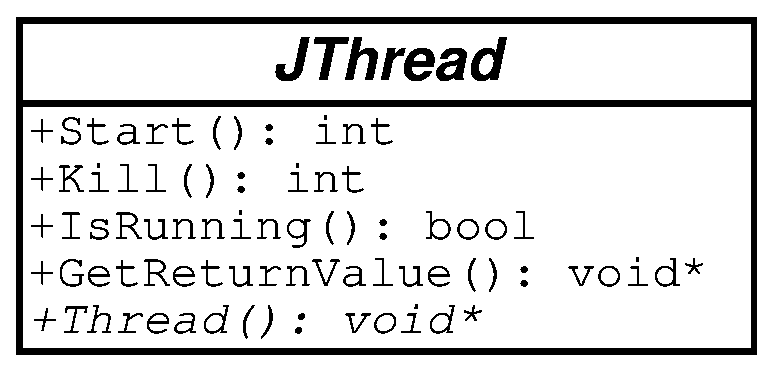
\includegraphics[width=0.35\linewidth]{images/manual/chapter4/class-jthread.eps}
			\caption{\tt JThread}
			\label{class-jthread}
		\end{figure}
		
		I also made an implementation of a mutex, called {\tt JMutex}. This class
		is represented in figure \ref{class-jmutex}. Before you can use the mutex,
		you must first call its {\tt Init} function. Then, you can lock and unlock
		the mutex by calling the member functions {\tt Lock} and {\tt Unlock}.
		\begin{figure}
			\center
			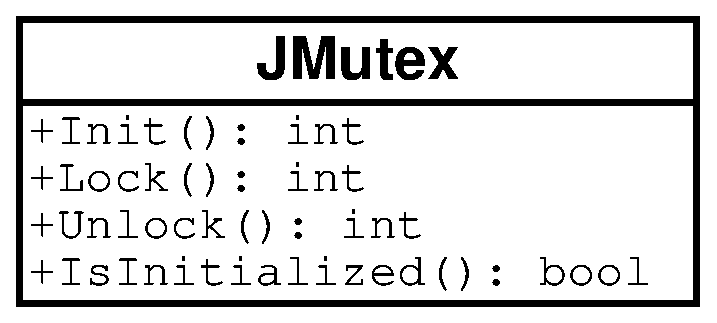
\includegraphics[width=0.35\linewidth]{images/manual/chapter4/class-jmutex.eps}
			\caption{\tt JMutex}
			\label{class-jmutex}
		\end{figure}
		
		\subsection{\tt JVOIPSampleConverter}
		
		When you're developing a component, you may need to convert the samples to
		another type, for example to a different sampling rate. To avoid having to
		implement such routines over and over again, I wrote an easy to use sample
		converter.
		
		The sample converter is implemented in the class {\tt JVOIPSampleConverter}.
		First, you have to set the conversion parameters by calling the function
		{\tt SetConversionParams}. Then, you can convert the samples by calling
		the {\tt Convert} member function. The syntax of these functions is like this:
		\begin{lstlisting}[frame=tb]{}
class JVOIPSampleConverter
{
public:
	int SetConversionParams(int sourcerate,
	                        bool sourcestereo,
	                        int sourcebytespersample,
	                        bool sourcesigned,
	                        bool sourceLittleEndian,
	                        int destrate,
	                        bool deststereo,
	                        int destbytespersample,
	                        bool destsigned,
	                        bool destLittleEndian);
	int Convert(unsigned char *sourcebuffer,int sourcelength,
	            unsigned char *destbuffer,int destlength);
};
	\end{lstlisting}

	When you call the {\tt Convert} function, it returns the actual number of
	bytes filled in in the destination buffer.
	
		\subsection{\tt JVOIPSimpleTimer}
		
		If you should need a simple timing module, you can use the class
		{\tt JVOIPSimpleTimer}. It does {\em not} time {\em exact} intervals, but it
		will make sure that the requested interval is attained {\em on average}.
		The class is depicted in figure \ref{class-jvoipsimpletimer}.If you compare 
		this figure with figure \ref{class-jvoipvoiceinput}, you'll see that
		{\tt JVOIPSimpleTimer} implements {\tt JVOIPSamplingTimer}. 
		\begin{figure}
			\center
			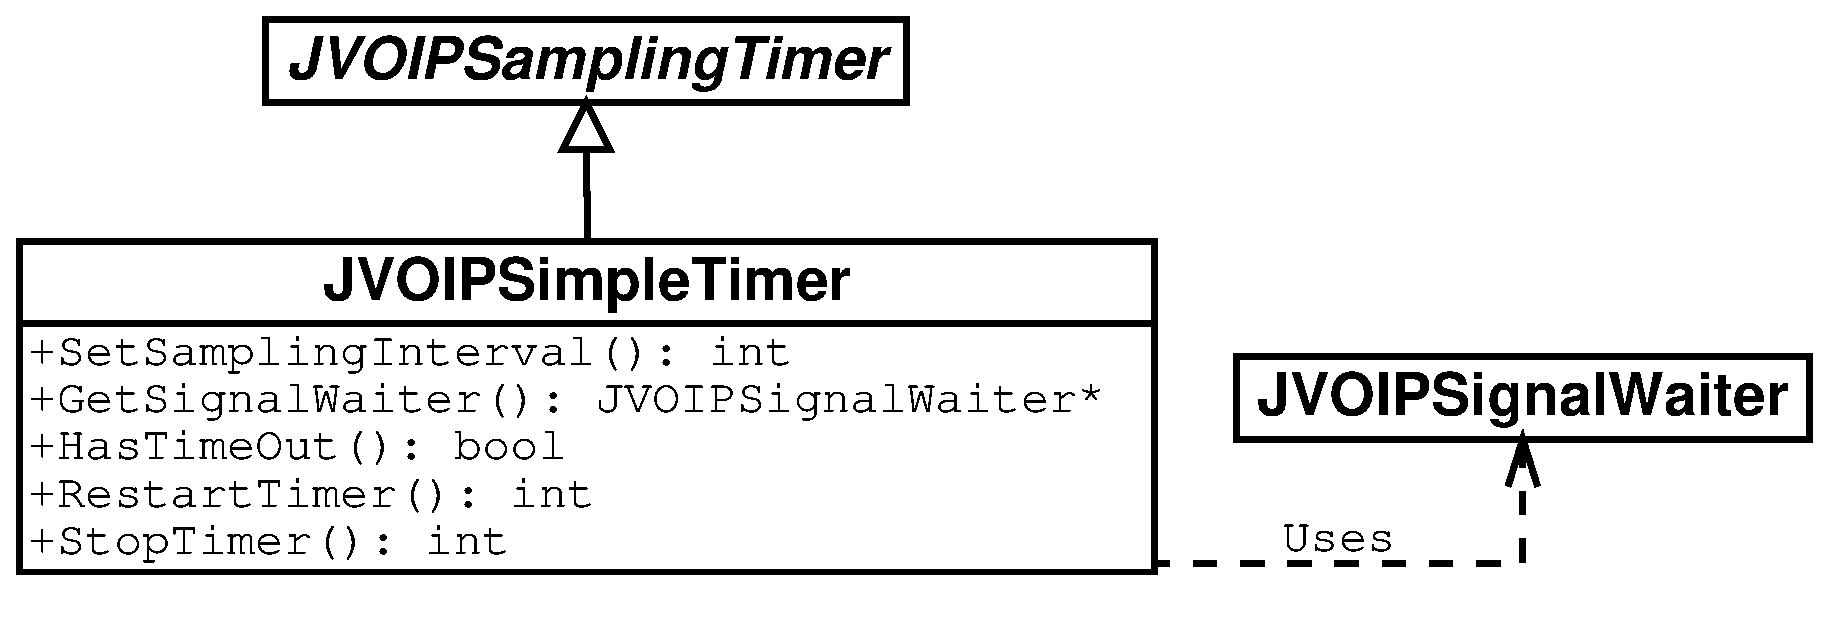
\includegraphics[width=0.7\linewidth]{images/manual/chapter4/class-jvoipsimpletimer.eps}
			\caption{\tt JVOIPSimpleTimer}
			\label{class-jvoipsimpletimer}
		\end{figure}
		
		{\tt JVOIPSimpleTimer} has two additional functions. The first is called
		{\tt Set\-Sampling\-In\-ter\-val}. As the name suggests, this function can be used
		to set the timeout interval of the timer. With the member function 
		{\tt StopTimer} you can -- as you might suspect -- stop the timer.
	
	\section{Voice input}
	
		\subsection{Required functions}
		
		To create a new voice input component you would need to create a class
		like this one:
		\begin{lstlisting}[frame=tb]{}
class MyInput : public JVOIPVoiceInput
{
public:
	MyInput(JVOIPSession *sess);
	~MyInput();
	int Init(int sampinterval, int inputsamprate, 
	         int inputbytespersample,
	         const JVOIPComponentParams *componentparams);
	int Cleanup();
	int StartSampling();
	void Reset();
	int GetSampleBlock(VoIPFramework::VoiceBlock *vb);
	JVOIPSamplingTimer *GetSamplingTimer();
	bool SupportsSampleInterval(int ival);
	bool SupportsInputSamplingRate(int irate);
	bool SupportsInputBytesPerSample(int inputbytespersample);
	int SetSampleInterval(int ival);
	int SetInputSamplingRate(int irate);
	int SetInputBytesPerSample(int inputbytespersample);

	int GetComponentState(JVOIPComponentState **compstate);
	int SetComponentState(JVOIPComponentState *compstate);
	
	std::string GetComponentName();
	std::string GetComponentDescription();
	std::vector<JVOIPCompParamInfo> *GetComponentParameters() 
	                                 throw (JVOIPException);
};
		\end{lstlisting}
		The sampling timer which is returned by your input component has to
		be managed completely by this class. For example, if you should allocate
		a timer dynamically when the component is initialized, you should probably
		delete it when the {\tt Cleanup} function is called.
		
		You could also implement the timer in the same class as the input module.
		Your component class would then inherit both {\tt JVOIPVoiceInput} and
		{\tt JVOIPSamplingTimer}. The {\tt GetSamplingTimer} member function would
		then simply return `{\tt this}'. This is the way that I implemented the 
		soundcard input module. The component did the timing based upon the 
		soundcard sample intervals.
		
		\subsection{Merging with the library}
		
		If you want to add your component to the library, you have to make modifications
		to two files: {\tt src/jvoipsessionparams.h} and {\tt src/jvoipsession.cpp}.
		
		In {\tt jvoipsessionparams.h} you have to add a type name for your component
		to the {\tt VoiceInputType} enumeration. For example, lets call it {\tt MyInputType}.
		
		Then, you have to make adjustments to {\tt jvoipsession.cpp}. In this file, you
		have to locate the {\tt JVOIPSession} member function {\tt ProcessInputType}. In
		this function, you'll find a switch statement. There, you'll have to add something
		like this:
		\begin{lstlisting}[frame=tb]{}
	case JVOIPSessionParams::MyInputType:
		voiceinput = new MyInput(this);
		break;
		\end{lstlisting}
	
	\section{Voice output}
	
		\subsection{Required functions}
		
		To create a new output component, you have to inherit a class from 
		{\tt JVOIPVoiceOutput}. The code below is a sample class definition; 
		it illustrates which member functions need to be implemented.
		\begin{lstlisting}[frame=tb]{}
class MyOutput : public JVOIPVoiceOutput
{
public:
	MyOutput(JVOIPSession *sess);
	~MyOutput();
	int Init(int sampinterval, int outputsamprate, 
	         int outputbytespersample, bool stereo,
	         const JVOIPComponentParams *componentparams);
	int Cleanup();
	int Play(VoIPFramework::VoiceBlock *vb);
	void Reset();
	bool SupportsSampleInterval(int ival);
	int SetSampleInterval(int ival);
	bool SupportsOutputSamplingRate(int orate);
	int SetOutputSamplingRate(int orate);
	bool SupportsOutputBytesPerSample(int outputbytespersample);
	int SetOutputBytesPerSample(int outputbytespersample);
	int SetStereo(bool s);
	
	int GetComponentState(JVOIPComponentState **compstate);
	int SetComponentState(JVOIPComponentState *compstate);
	
	std::string GetComponentName();
	std::string GetComponentDescription();
	std::vector<JVOIPCompParamInfo> *GetComponentParameters()
	                                 throw (JVOIPException);
};
		\end{lstlisting}

		\subsection{Merging with the library}

		To merge your new output component with the library, you have to follow a 
		similar procedure as with the input component. 
		
		First, you have to edit the file {\tt src/jvoipsessionparams.h} and add a new
		output type to the {\tt VoiceOutputType} enumeration. Lets call this type 
		{\tt MyOutputType}.
		
		The next step is to edit the file {\tt src/jvoipsession.cpp}. There, you have
		to alter the code of the {\tt JVOIPSession} member function 
		{\tt ProcessOutputType}
		\begin{lstlisting}[frame=tb]{}
	case JVOIPSessionParams::MyOutputType:
		voiceoutput = new MyOutput(this);
		break;
		\end{lstlisting}

	\section{Localisation}

		\subsection{Required functions}
		
		If you want to implement a new localisation scheme, you can use one of two 
		approaches: you can inherit a class from {\tt JVOIPLocalisation} or you 
		can inherit a class from {\tt JVOIP\-Session\-Localisation}.
		
		If you want to add a new localisation component to the library, it should
		be inherited from {\tt JVOIPSessionLocalisation}. This ensures interoperability
		between the different localisation schemes of the library.
		
			\subsubsection{Inheriting from {\tt JVOIPSessionLocalisation}}
			
			If you inherit from {\tt JVOIPSessionLocalisation}, your component will have
			a class definition like this:
			\begin{lstlisting}[frame=tb]{}
class MySessionLocalisation : public JVOIPSessionLocalisation
{
public:
	MySessionLocalisation(JVOIPSession *sess);
	~MySessionLocalisation();
	int Init(int outputsamprate, int outputbytespersample, 
	         const JVOIPComponentParams *componentparams);
	int Cleanup();
	int Create3DEffect(double local_x, double local_y, 
	                   double local_z, double righteardir_x,
	                   double righteardir_y, double righteardir_z,
					   double frontdir_x, double frontdir_y,
					   double frontdir_z, double updir_x,
					   double updir_y, double updir_z,
	                   double remote_x, double remote_y, 
	                   double remote_z,
	                   VoIPFramework::VoiceBlock *vb,
	                   VoIPFramework::VOIPuint64 sourceid);
	
	bool SupportsOutputSamplingRate(int orate);
	int SetOutputSamplingRate(int orate);
	bool SupportsOutputBytesPerSample(int outputbytespersample);
	int SetOutputBytesPerSample(int outputbytespersample);
	
	int GetComponentState(JVOIPComponentState **compstate);
	int SetComponentState(JVOIPComponentState *compstate);
	
	std::string GetComponentName();
	std::string GetComponentDescription();
	std::vector<JVOIPCompParamInfo> *GetComponentParameters() 
	                                 throw (JVOIPException);
};
			\end{lstlisting}
			
			In this approach, you only have to worry about calculating the 3D effects based
			upon the positional info in the arguments of {\tt Create3DEffect}. This 
			information is obtained by the class' parent {\tt JVOIPSessionLocalisation} from
			the {\tt JVOIPSession} overridable functions {\tt RetrieveOwnPosition}, 
			{\tt EncodeOwnPosition} and {\tt DecodePositionalInfo}.
			
			\subsubsection{Inheriting from {\tt JVOIPLocalisation}}
			
			If you need to have more control over the storage and content of the positional
			information, you can inherit your new localisation class from {\tt JVOIPLocalisation}.
			Your class would then look something like this:
			\begin{lstlisting}[frame=tb]{}
class MyLocalisation : public JVOIPLocalisation
{
	MyLocalisation(JVOIPSession *sess);
	~MyLocalisation();
	int Init(int outputsamprate, int outputbytespersample, 
	         const JVOIPComponentParams *componentparams);
	int Cleanup();
	int Add3DInfo(VoIPFramework::VoiceBlock *vb);
	int Create3DEffect(VoIPFramework::VoiceBlock *vb,
	                   VoIPFramework::VOIPuint64 sourceid);
	
	bool SupportsOutputSamplingRate(int orate);
	int SetOutputSamplingRate(int orate);
	bool SupportsOutputBytesPerSample(int outputbytespersample);
	int SetOutputBytesPerSample(int outputbytespersample);
	
	int GetComponentState(JVOIPComponentState **compstate);
	int SetComponentState(JVOIPComponentState *compstate);
	
	std::string GetComponentName();
	std::string GetComponentDescription();
	std::vector<JVOIPCompParamInfo> *GetComponentParameters() 
	                                 throw (JVOIPException);
};
			\end{lstlisting}

		\subsection{Merging with the library}

		As I explained above, if you want to add a new localisation component to
		the library, it should be derived from {\tt JVOIPSessionLocalisation}.
		The procedure is the same as with the previous components.
		
		First, edit the file {\tt src/jvoipsessionparams.h}. There, you have to
		add a new localisation type to the {\tt LocalisationType} enumeration.
		For example, lets call it {\tt My\-Session\-Loca\-li\-sa\-tion}.
		
		In {\tt src/jvoipsession.cpp}, you have to alter the {\tt JVOIPSession}
		member function {\tt ProcessLocalisationType}. Inside the switch statement
		you have to add a piece of code like this:
		\begin{lstlisting}[frame=tb]{}
	case JVOIPSessionParams::MySessionLocalisation:
		localisation = new MySessionLocalisation(this);
		break;                                                          
		\end{lstlisting}

	\section{Compression}

		\subsection{Required functions}

		To create a new compression module, you have to derive a class from
		{\tt JVOIP\-Com\-pres\-sion\-Mo\-dule}. Your class would then look something
		like this:
		\begin{lstlisting}[frame=tb]{}
class MyCompressionModule : public JVOIPCompressionModule
{
public:
	MyCompressionModule(JVOIPSession *sess);
	~MyCompressionModule();
	int InitCompressor(int sampinterval, int inputsamprate, 
	                   int inputbytespersample,
	                   const JVOIPComponentParams *componentparams);
	int CleanupCompressor();
	int InitDecompressor();
	int CleanupDecompressor();

	int Compress(VoIPFramework::VoiceBlock *vb);
	int Decompress(VoIPFramework::VoiceBlock *vb,
	               VoIPFramework::VOIPuint64 sourceid);

	bool SupportsSampleInterval(int ival);
	int SetSampleInterval(int ival);
	bool SupportsInputSamplingRate(int irate);
	int SetInputSamplingRate(int irate);
	bool SupportsInputBytesPerSample(int inputbytespersample);
	int SetInputBytesPerSample(int inputbytespersample);

	int GetComponentState(JVOIPComponentState **compstate);
	int SetComponentState(JVOIPComponentState *compstate);

	std::string GetComponentName();
	std::string GetComponentDescription();
	std::vector<JVOIPCompParamInfo> *GetComponentParameters() 
	                                 throw (JVOIPException);
};
		\end{lstlisting}
		
		\subsection{Merging with the library}
		
		Adding a new compression component to the library is a bit more work than
		adding an other component type. Like with the other types, you have to edit
		the file {\tt src\-/jvoip\-ses\-sion\-pa\-rams.h} and add a new type to the 
		{\tt CompressionType} enumeration. Lets call this type {\tt My\-Com\-pres\-sion}
		
		Then, you have to add a new major compression type identifier to 
		{\tt src/\-lib\-com\-po\-nents/\-base/\-jvoip\-com\-pres\-sion.h}. Suppose we call this 
		identifier {\tt JVOIP\-COM\-PRES\-SION\-TYPE\_MAJOR\_MY\-COM\-PRES\-SION}.
		
		In the same file, you also find the class definition of {\tt JVOIPCompression}.
		In the {\tt private} section, you have to add a new member variable, like this:
		\begin{lstlisting}[frame=tb]{}
	JVOIPCompressionModule *mycompr_compmod;
		\end{lstlisting}

		Next, you have to edit the file {\tt src/libcomponents/base/jvoipcompression.cpp}.
		In the {\tt Decompress} member function of {\tt JVOIPCompression}, you'll find a
		switch statement. There you have to add a piece of code like this:
		\begin{lstlisting}[frame=tb]{}
	case JVOIPCOMPRESSIONTYPE_MAJOR_MYCOMPRESSION:
		status = mycompr_compmod->Decompress(vb,sourceid);
		if (status < 0)
			return status;
		break;
		\end{lstlisting}

		The following step is to modify the {\tt ProcessCompressionType} member function.
		Here, you also have to alter the switch statement by adding a piece of code
		like this:
		\begin{lstlisting}[frame=tb]{}
	case JVOIPSessionParams::MyCompression:
		*compmod = mycompr_compmod;
		*majorcomptype = JVOIPCOMPRESSIONTYPE_MAJOR_MYCOMPRESSION;
		break;
		\end{lstlisting}

		Then you have to change the {\tt InitModules} function. Here's where your
		component will be allocated. First, you have to set your component to {\tt NULL},
		{\em before} any {\tt CREATE\_AND\_INIT} calls:
		\begin{lstlisting}[frame=tb]{}
	mycompr_compmod = NULL;
		\end{lstlisting}

		Next, you have to create and initialize your component. This can easily be done
		by using the {\tt CREATE\_AND\_INIT} macro. You have to call it {\em before} the
		user defined component is initialized.
		\begin{lstlisting}[frame=tb]{}
	CREATE_AND_INIT(mycompr_compmod,MyCompressionModule);
		\end{lstlisting}

		Finally, you have to modify the {\tt DeleteModules} member function. In this function,
		you have to add code to delete your component. In our example, it would be something
		like this:
		\begin{lstlisting}[frame=tb]{}
	if (mycompr_compmod)
		delete mycompr_compmod;
		\end{lstlisting}

	\section{Mixer}

		\subsection{Required functions}

		If you want to make a new mixer component, you have to derive your class from
		{\tt JVOIPMixer}. This class would then look something like this:
		\begin{lstlisting}[frame=tb]{}
class MyMixer : public JVOIPMixer
{
public:
	MyMixer(JVOIPSession *sess);
	~MyMixer();
	int Init(int sampinterval, int outputsamprate, 
	         int outputbytespersample, bool stereo,
	         const JVOIPComponentParams *componentparams);
	int Cleanup();

	int AddBlock(VoIPFramework::VoiceBlock *vb,
	             VoIPFramework::VOIPuint64 sourceid);
	
	int GetSampleBlock(VoIPFramework::VoiceBlock *vb);
	int GetSampleOffset(VoIPFramework::VOIPdouble *offset);
	
	bool SupportsSampleInterval(int ival);
	int SetSampleInterval(int ival);
	bool SupportsOutputSamplingRate(int orate);
	int SetOutputSamplingRate(int orate);
	bool SupportsOutputBytesPerSample(int outputbytespersample);
	int SetOutputBytesPerSample(int outputbytespersample);
	int SetStereo(bool s);

	int GetComponentState(JVOIPComponentState **compstate);
	int SetComponentState(JVOIPComponentState *compstate);
	
	std::string GetComponentName();
	std::string GetComponentDescription();
	std::vector<JVOIPCompParamInfo> *GetComponentParameters() 
	                                 throw (JVOIPException);
};
		\end{lstlisting}

		\subsection{Merging with the library}

		Merging with the library is easy. First, you edit the file 
		{\tt src/jvoipsessionparams.h}. There, you have to add a new type to the
		{\tt MixerType} enumeration. Suppose you call this type {\tt MyMixerType}.

		Then, you have to modify the file {\tt src/jvoipsession.cpp}. In the
		{\tt JVOIPSession} member function {\tt ProcessMixerType}, you'll find
		a switch statement. There, you have to insert a piece of code like this:
		\begin{lstlisting}[frame=tb]{}
	case JVOIPSessionParams::MyMixerType:
		mixer = new MyMixer(this);
		break;
		\end{lstlisting}

	\section{Transmission}

		\subsection{Required functions}

		When you want to make a new transmission component, you have to derive
		a class from {\tt JVOIPTransmission}. Your class definition would then
		look like this:
		\begin{lstlisting}[frame=tb]{}
class MyTransmission : public JVOIPTransmission
{
public:
	MyTransmission(JVOIPSession *sess);
	~MyTransmission();
	
	int Init(int sampinterval, int inputsamprate, 
	         int inputbytespersample, 
	         const JVOIPComponentParams *componentparams);
	int Cleanup();
	void Reset();
	
	int SendBlock(VoIPFramework::VoiceBlock *vb);
	int StartVoiceSourceIteration();
	void EndVoiceSourceIteration();
	bool GotoFirstVoiceSource();
	bool GotoNextVoiceSource();
	VoIPFramework::VOIPuint64 GetVoiceSourceID();
	int GetSampleBlock(VoIPFramework::VoiceBlock *vb);
	int Poll();
	bool SourceHasMoreData();
	int SetSampleOffset(VoIPFramework::VOIPdouble offset);
	
	bool AddDestination(JVOIPuint32 destip,
	                    JVOIPuint16 destportbase);
	bool DeleteDestination(JVOIPuint32 destip,
	                       JVOIPuint16 destportbase);
	void ClearDestinations();

	bool SupportsMulticasting();	
	bool JoinMulticastGroup(JVOIPuint32 mcastip);
	bool LeaveMulticastGroup(JVOIPuint32 mcastip);
	void LeaveAllMulticastGroups();

	bool SupportsReceiveType(JVOIPSessionParams::ReceiveType rt);
	bool SetReceiveType(JVOIPSessionParams::ReceiveType rt);
	bool AddToAcceptList(JVOIPuint32 ip,
	                     JVOIPuint16 port = JVOIP_ALLPORTS);
	bool DeleteFromAcceptList(JVOIPuint32 ip,
	                          JVOIPuint16 port = JVOIP_ALLPORTS);
	void ClearAcceptList();
	bool AddToIgnoreList(JVOIPuint32 ip,
	                     JVOIPuint16 port = JVOIP_ALLPORTS);
	bool DeleteFromIgnoreList(JVOIPuint32 ip,
	                          JVOIPuint16 port = JVOIP_ALLPORTS);
	void ClearIgnoreList();

	bool SupportsSampleInterval(int ival);
	int SetSampleInterval(int ival);
	bool SupportsInputSamplingRate(int irate);
	int SetInputSamplingRate(int irate);
	bool SupportsInputBytesPerSample(int inputbytespersample);
	int SetInputBytesPerSample(int inputbytespersample);

	int GetComponentState(JVOIPComponentState **compstate);
	int SetComponentState(JVOIPComponentState *compstate);
	
	std::string GetComponentName();
	std::string GetComponentDescription();
	std::vector<JVOIPCompParamInfo> *GetComponentParameters() 
	                                 throw (JVOIPException);
};
		\end{lstlisting}

		\subsection{Merging with the library}

		To add your new component to the library, you have to follow the same
		procedure as with most of the other components.

		First, you have to edit {\tt src/jvoipsessionparams.h}. In this file,
		you have to add a type to the {\tt TransmissionType} enumeration.
		Let's call this {\tt MyTransmissionType}.

		Next, you have to edit {\tt src/jvoipsession.cpp}. In the {\tt JVOIPSession}
		member function {\tt ProcessTransmissionType}, you have to add some code to
		the switch statement. In our example:
		\begin{lstlisting}[frame=tb]{}
	case JVOIPSessionParams::MyTransmissionType:
		transmission = new MyTransmission(this);
		break;
		\end{lstlisting}

